\section{Experimental Setup}

The experimental setup consists of a Stokes’ viscosity measurement device (see
Figure 1) filled with castor oil in which motion of small metal balls will be
observed.

Measurements of various physical quantities in the experiment are performed with
a number of measurement devices: micrometer, calliper, densimeter, electronic
scales, stopwatch, and thermometer.

\begin{figure}[H]
\centering
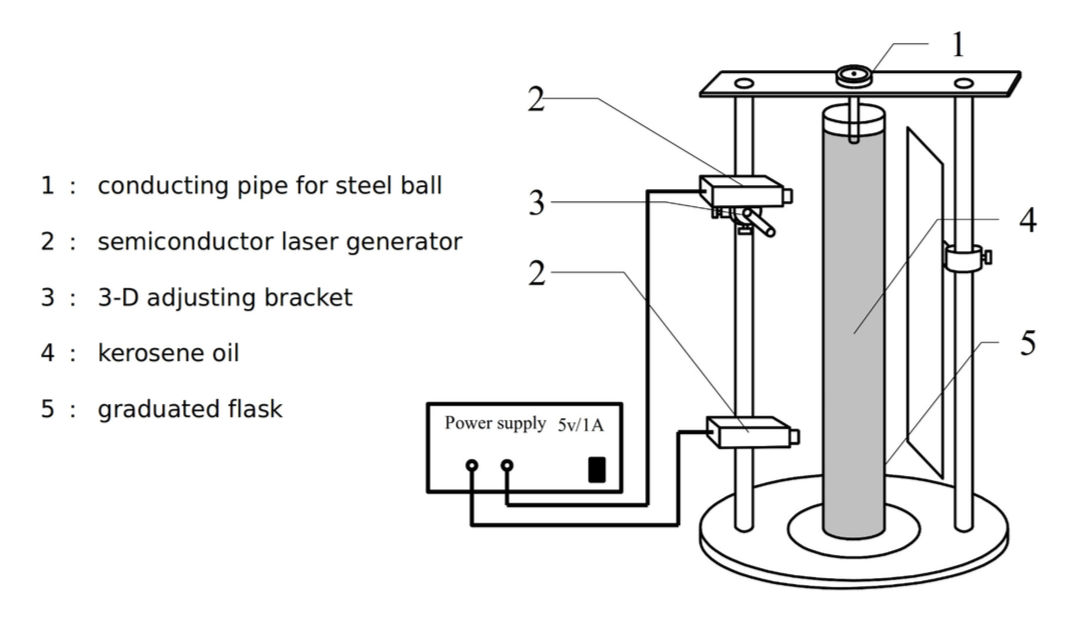
\includegraphics[width=12cm]{fig/p1}
\caption{Stokes viscosity measurement apparatus}
\end{figure}

